\section{org::simtk::molecularstructure::Nucleic\-Acid Class Reference}
\label{classorg_1_1simtk_1_1molecularstructure_1_1_nucleic_acid}\index{org::simtk::molecularstructure::NucleicAcid@{org::simtk::molecularstructure::NucleicAcid}}
A single molecule of {\bf DNA}{\rm (p.\,\pageref{classorg_1_1simtk_1_1molecularstructure_1_1_d_n_a})} or {\bf RNA}{\rm (p.\,\pageref{classorg_1_1simtk_1_1molecularstructure_1_1_r_n_a})}.  


Inheritance diagram for org::simtk::molecularstructure::Nucleic\-Acid::\begin{figure}[H]
\begin{center}
\leavevmode
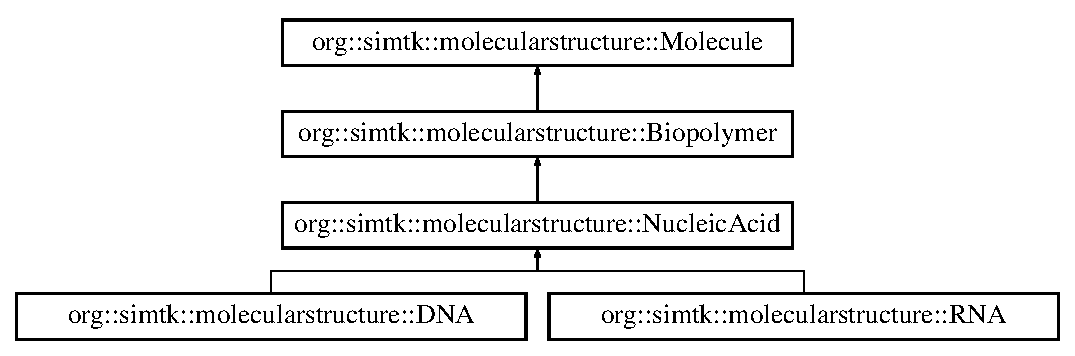
\includegraphics[height=4cm]{classorg_1_1simtk_1_1molecularstructure_1_1_nucleic_acid}
\end{center}
\end{figure}


\subsection{Detailed Description}
A single molecule of {\bf DNA}{\rm (p.\,\pageref{classorg_1_1simtk_1_1molecularstructure_1_1_d_n_a})} or {\bf RNA}{\rm (p.\,\pageref{classorg_1_1simtk_1_1molecularstructure_1_1_r_n_a})}. 

\begin{Desc}
\item[Author:]Christopher Bruns \end{Desc}




The documentation for this class was generated from the following file:\begin{CompactItemize}
\item 
C:/cygwin/home/cmbruns/eclipse/vtkjava/org/simtk/molecularstructure/Nucleic\-Acid.java\end{CompactItemize}
